\documentclass{article}

% For revision control
\usepackage{rcs-multi}
\rcsid{$Id$}
\rcsid{$Header$}
\rcskwsave{$Author$}
\rcskwsave{$Date$} 
\rcskwsave{$Revision$}
\rcsRegisterAuthor{devangel}{Dennis J. Evangelista}

% I typically use these
\usepackage{graphicx}
\usepackage[usenames,dvipsnames]{color}
\usepackage{makeidx}
\usepackage{siunitx}

% PDF metadata
\usepackage{hyperref}
\hypersetup{pdftitle={Stunned mice and splashed horses: Rethinking the falling animal death curve}}
\hypersetup{pdfauthor={J. Alphabetical, D. Evangelista, K. Jayaram, T. Libby and D. Springthorpe}}
\hypersetup{pdfsubject={biology}}
\hypersetup{pdfkeywords={biomechanics, evolution, falling animal death curve, damage, mortality, LD50, falling}}
\hypersetup{colorlinks=true,citecolor=Violet,linkcolor=Blue,urlcolor=Red}

% Biology style references
\usepackage[round]{natbib}
\setcitestyle{authoryear, round, comma, aysep={;}, yysep={,}, notesep={, }}
\bibliographystyle{apalike}

% Genus and species names
\newcommand{\Homosapiens}{\emph{Homo sapiens}}







\title{Stunned mice and splashed horses:  rethinking the falling animal death curve}
\author{Joe Alphabetical, Dennis Evangelista, Kaushik Jayaram,\\ Tom Libby, Dwight Springthorpe}
\date{\today}

\begin{document}
\maketitle

\begin{abstract}
This project will examine the impact resistance of invertebrates.  Animals will be subjected to a blunt force impact using two types of whole-body tests: (1) a drop test in which the animal is dropped in air from a height; and (2) a falling weight test in which a large, blunt weight is dropped on a stationary animal.  Injuries and survival will be recorded, and the relationships between likelihood of death, impact energy, impulse, and force will be determined.
\end{abstract}

\section{Introduction}
Impact resistance is an important physical constraints on organisms, ecology, and evolution, especially during locomotion, predator-prey interactions \citep{Patek:2005}, male-male combat and display, transition onto land, or evolution of flight and gliding.  Despite the biological importance of impact resistance, it is usually only quantified in terms of the energy/volume to fracture material specimens.  Such materials characterizations are valuable, but lack consideration of the the effects of shape, composite structure, and behavior.  

In engineering practice, the ability of a design to withstand impact is usually determined from various forms of drop or shock tests.  For vertebrates, only limited whole-body data is available from medical and veterinary pathology and anthropology, specifically, high-rise falls in humans \citep{Westman:2007, Goren:2004, DeHaven:1942}, dogs \citep{Gordon:1993}, cats \citep{Vnuk:2004}, chimpanzees \citep{Goodall:1986}.  Among invertebrates, sparse data exist from bird drops of clams and cockles \citep{Marron:1982} and falling-weight tests on urchins \citep{Strathmann:1981}.  The lack of data is puzzling, as the impact energy required to fracture a shell is one direct measure of the cost to predators. 

The results of this project will be paired with other efforts to compile similar data for vertebrates in a master curve, to explore scaling differences among groups.  A preliminary version of this curve is attached.  Initial hypotheses are: (1) Scaling will reduce into one or a few physically-meaningful quantities, for example, mass specific impact energy (J/kg), that are invariant across size.  (2) Scaling for animals with endoskeletons will be different from those with exoskeletons.  (3) Scaling for mobile animals will be different from scaling for sessile animals, reflecting relative costs of transport, armor, and support.  (4) Some organisms will exhibit higher relative resistance to impact, through use of brakes or energy absorbing structures.  These will be made apparent through the scaling.

\section{Materials and methods}
Drop tests will be conducted from several heights up to 4 stories and will be filmed to obtain velocity.  Building safety will require drop tests to be performed under the supervision of the building manager and during a narrow window of time.  Falling weight tests will be conducted using a commercially available impact/Charpy testing machine, or using or a similar design pendulum or falling weight rig, in a manner similar to \citet{Strathmann:1981}.  Falling weight tests will be filmed at high speed to observe impact velocity, and the rig will be instrumented to record impact force.  Specimens will be kept in a tank until immediately before testing.  Specimens will be weighed and photographed before and after dropping, and scored based on mechanical integrity (holes, cracks, lost limbs, etc.), behavioral effects, or death.  Forces, impact energy, height, velocity, impulse, mass, and damage and death rates will be analyzed in Matlab to obtain statistics and allometric regressions.  Substrate effects will be determined using resilience tests (dropped rubber ball), to estimate how much energy is absorbed by the ground versus how much must be absorbed by the body.  By testing in air, fluid effects can be more easily subtracted.  Results can be applied to movements in water using widely available data on drag, added mass, and fluid forcing. 

\section{Results}

\begin{figure}
\begin{center}
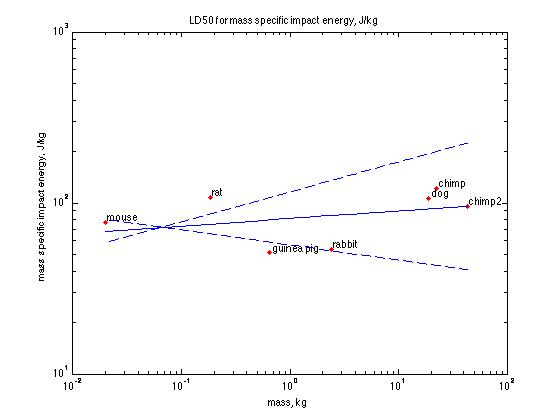
\includegraphics[width=\textwidth]{figures/current-death-curve.jpg}
\end{center}
\caption{Current death curve}
\end{figure}

\begin{figure}
\begin{center}
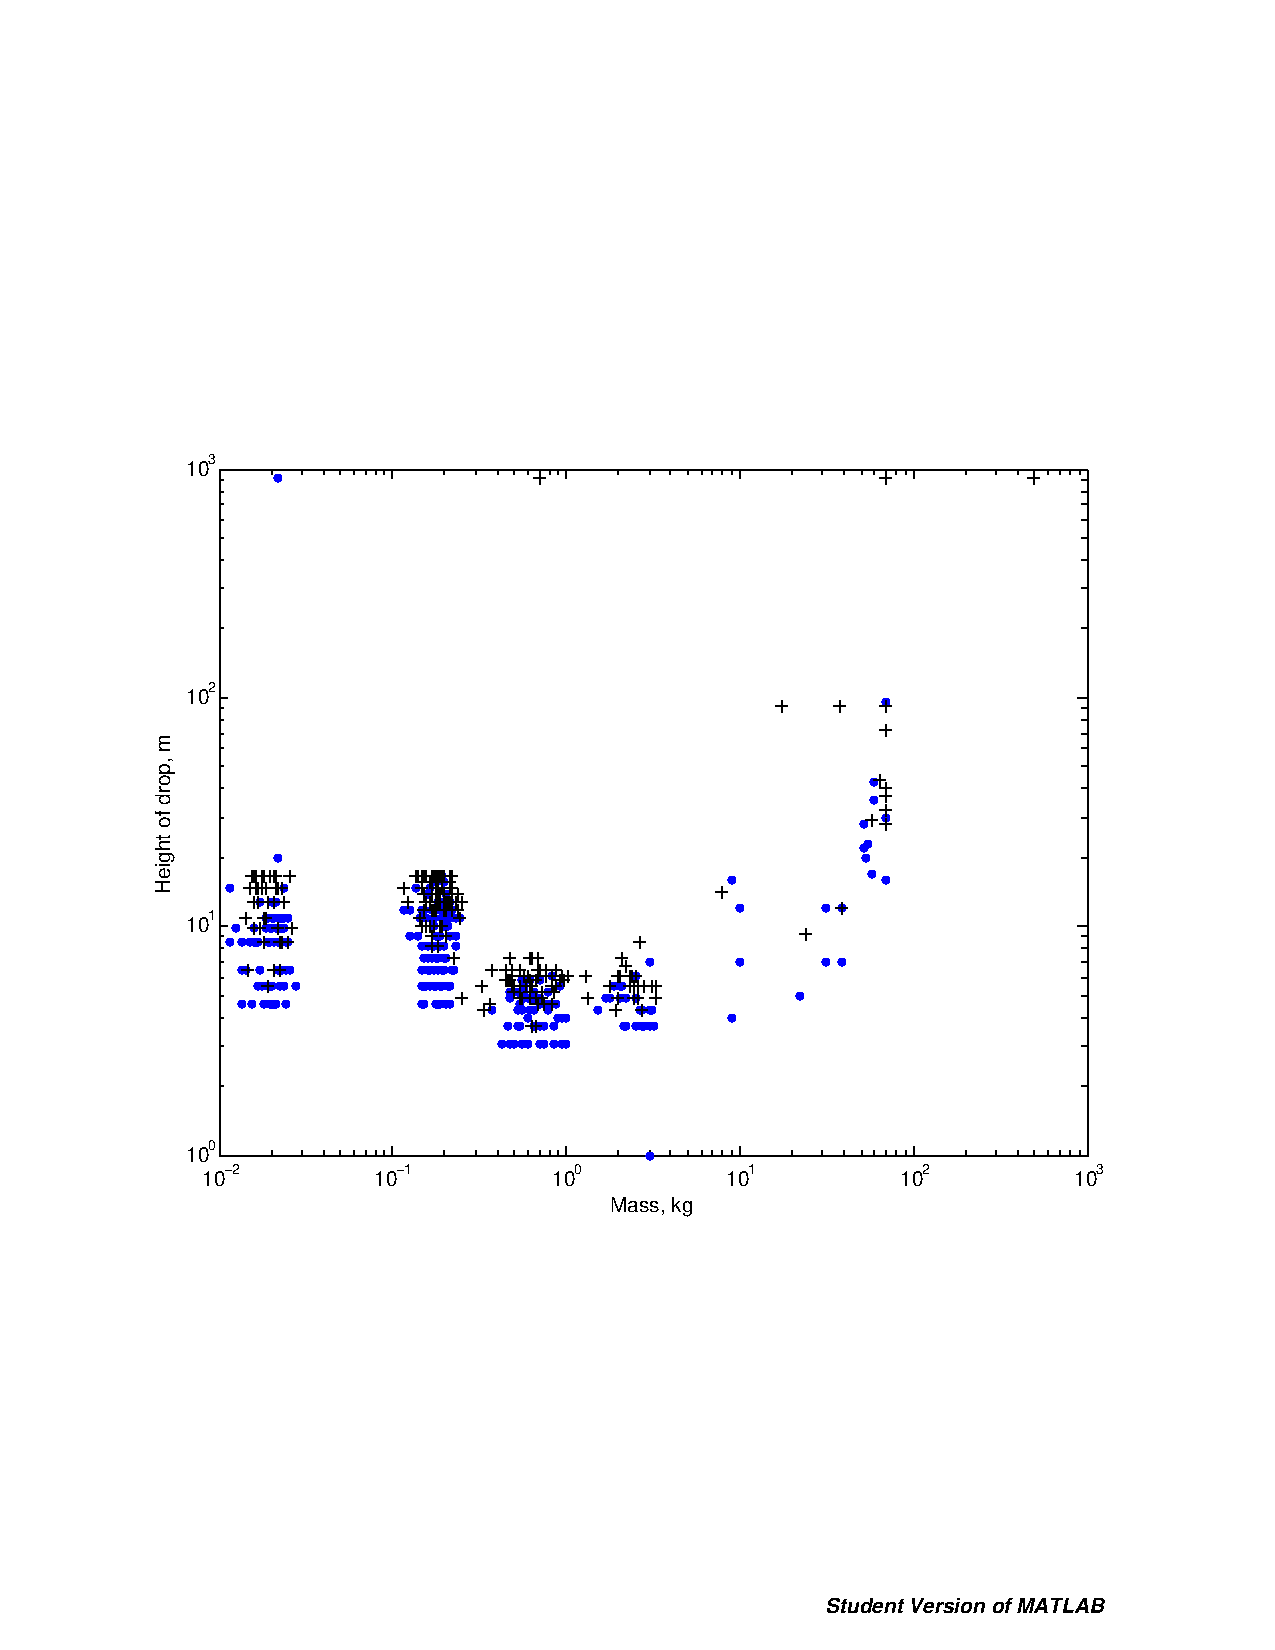
\includegraphics[width=\textwidth]{figures/raw-death-curve-height.pdf}
\end{center}
\caption{Current death curve}
\end{figure}

\begin{table}
\begin{center}
\begin{tabular}{lr}
See dog run & run \\
See cat scratch & fever \\
\end{tabular}
\end{center}
\caption{Example table}
\end{table}

\section{Discussion}
%\section{List of symbols}
%\section{Appendix}
\section*{Acknowledgements}

\bibliography{references/falling}

\end{document}
